%chktex-file 46 
%%turn off the syntax check on $...$
\documentclass[a4paper,fleqn]{cas-sc}% fleqn stands for "flush left equations"
%%%%%%%%%%%%%%% Declare Package: %%%%%%%%%%%%%
\usepackage[authoryear,longnamesfirst]{natbib}
\usepackage{ragged2e}% Align macro package
\usepackage{amsmath,amssymb}
%%% Nomenclature packages %%%%%%%%%
\usepackage{framed,multicol}% frame and multi-column package in the double column for nomenclature
\usepackage{nomencl}% use nomenclature package
\makenomenclature
\setlength{\nomitemsep}{-\parskip} % Baseline skip between items
\renewcommand*\nompreamble{\begin{multicols}{2}}
\renewcommand*\nompostamble{\end{multicols}}
%%%%%%%%%%%%%%%%%%%%%%%%%%%%%%%%%%%%%%%%%%%%%%%%%%
\graphicspath{{Figures/}}% the path of graphs1
% \usepackage{bm}% bold font special for math formulas
\usepackage[name=Fig,labelsep=period]{caption}
% \usepackage[raggedright,nooneline,FIGTOPCAP]{subfigure}% need to call both packages: subcaption and caption at the same time
\usepackage{setspace}
\DeclareMathOperator\dif{d\!}% the derivative operator d
\usepackage{xfrac}% small fraction, for example 1/2
\usepackage{multirow,booktabs} %three-line table
\usepackage{array} % fixed width and auto newline(wrap) as well centering
\usepackage{callouts}
\usepackage{microtype}% improve the intervals between words to make typing more beautiful
\usepackage{lineno,hyperref}% display line number, use hyper reference
\usepackage{nameref}

%%%%%%%%%%%%%% Title and author: %%%%%%%%%%%%%
\begin{document}
\let\WriteBookmarks\relax
\def\floatpagepagefraction{1}
\def\textpagefraction{.001}
\shorttitle{Unequal planet load sharing}
\shortauthors{Feng et~al.}
\title[mode = title]{A vibration signal model of planetary gearboxes with unequal load sharing among planets}
\author[1]{Haoqun Ma}[type=editor]
\address[1]{University of Science and Technology Beijing, No.30, Xueyuan Road, Haidian District, Beijing.}
\author[1]{Zhipeng Feng}[orcid=0000-0002-3403-4386]
\cormark[1]
\cortext[cor1]{Corresponding author}%
\ead{fengzp@ustb.edu.cn}%
% 
%%%%%%%%%%%%%% Abstract %%%%%%%%%%%%%%%%%%%%%%
\begin{abstract}
    Planetary gearboxes feature large transmission ratios within compact volumes, because they can divide the input torque load into several paths through parallel planets. Unevenly load sharing among planets lead to inefficiency and accelerating fatigue. This paper establishes a vibration signal model to describe how the uneven distribution of planet loads affects the vibration signal composition. Compared with fixed shaft bearings, planet bearings are more prone to faults due to its excessive load. We also establish a vibration signal of planet bearing faults along with the uneven distribution of planet loads. Planet bearing faults are more difficult to diagnose due to abundant modulation sidebands arising from the unequal load sharing among planets. Numerical simulation and experimental substations agrees with the proposed theoretical model.
\end{abstract}
%%%%%%%%%%%%%%%%% Highlights %%%%%%%%%%%%%%%%%%%%%%
\begin{highlights}
    \item Vibration signal model of equal load sharing among planets
    \item Influence of gear meshing vibration, transfer path effects and natural frequency
    \item Analytical expression of Fourier spectrum 
    \item Explanation on spectral configuration arisen from different factors
\end{highlights}
%%%%%%%%%%%%%%%% keywords %%%%%%%%%%%%%%%%%%
\begin{keywords}
    Unequal load sharing \sep\ Planetary gearbox \sep\ Signal model \sep\ Fault diagnosis
\end{keywords}
    
%%%%%%%%%%%%%% Begin document: %%%%%%%%%%%%%%%
\maketitle
%%%%%%%%%%%%%%% Custom commands: %%%%%%%%%%%%
\setcitestyle{square}
\def\degree{${}^{\circ}$}
%%%%%%%%%%%%%%% Introduction %%%%%%%%%%%%%%%%
\section{Introduction}
\par Planets split power transmitted from the input sun gear into paralleled paths so that planetary gearboxes can withstand heavy load in a compact volume. While the special structure bring about unequal load sharing among planets.
%%%%%%%%%%%%%%% References %%%%%%%%%%%%%%%%%
%%%%%%%%%%%%%%% Principle %%%%%%%%%%%%%%%%
\section{Signal model}
\begin{enumerate}[1.]
    \item Planetary gearboxes have different configuration with similar layouts.
    \item In this paper, we only consider the case where ring gear is fixed. (refer to the paper mentioning the sun or carrier as the fixed central part)
    \item The vibration sensor is mounted on the stationary ring gear.
    \item The vibration mainly origins the the time-varying stiffness gear meshing. When the planet gears engage with the ring gear or sun gear, the number of the involved tooth varies with the relative rotation between gears. Thus, their contact stiffness changes at the same time. If the transmission load proximately remain constant, this system is pure parametric excited. (Add a reference about instability) 
    \item Specially, the torque load transferred from the central components in planetary gearboxes is split into parallel paths formed by the planets. Because of the inevitable manufacturing and assembling errors of pinholes or bearings, there are usually differences in the position of pinholes and the shape of planets. The load sharing among planets is non-uniform (collect other reasons from the Sigh's paper).
    \item Another common phenomenon in planetary gearboxes is the difference in meshing phases between ring-planet and sun-planet. When this situation coincides with the load sharing inequality, a complex couple mechanism of time-varying load sharing emerges, rising extra vibrations.
    \item For an individual planet, the vibration signal model can be written as
    \begin{equation}
        J \cdot \ddot{\theta}(t) + k(t) \cdot \left[\theta(t)-L(t) \right] = 0,
    \end{equation}
    where \(J\) is the rotational inertia of machine, \(\theta(t)\) is the shaft angular, \(\ddot{\theta}(t)\) is the rotational acceleration, \(k(t)\) is time-varying meshing stiffness, \(L(t)\) is the external load.
    \item Taking all planets into account, the above vibration model can be revised as
    \begin{equation}
        J \cdot \ddot{\theta}(t) + \sum^{M}_{i=1} \left\{ k_i(t) \cdot \left[\theta(t)-L(t)+\epsilon_i \right] \right\} = 0,
    \end{equation}
    where \(M\) is the number of planets, \(k_i(t)\) is the meshing stiffness of \(i\)-th planet, \(\epsilon_i\) is the angular shift away from its normal position of \(i\)-th planet (here we assume \(\epsilon_2\neq 0\)). A translational spring-mass system illustrate the above vibration model in Fig. \ref{fig:vibration_system_of_spring_mass}.
    %%%%%%%%%%%%%%%%% nomenclature Display %%%%%%%%%%%%
\begin{table*}[!t] 
    \begin{framed} 
        \printnomenclature
    \end{framed}
\end{table*}
\nomenclature{\(f_{\rm m}\)}{gear meshing frequency}
\nomenclature{\(f_{\rm c}\)}{carrier rotation frequency}
\nomenclature{\(J\)}{inertia moment}
\nomenclature{\(k(t)\)}{stiffness}
\nomenclature{\(L_i\)}{load sharing ratio of the \(i\)-th planet}
\nomenclature{\(k_e\)}{effective support stiffness concerning both the bearing and gear meshing}
\nomenclature{\(r_s\)}{sun gear pitch radius}
\nomenclature{\(T_s\)}{total torque applied on input sun gear}
    \begin{figure*}
        \centering
        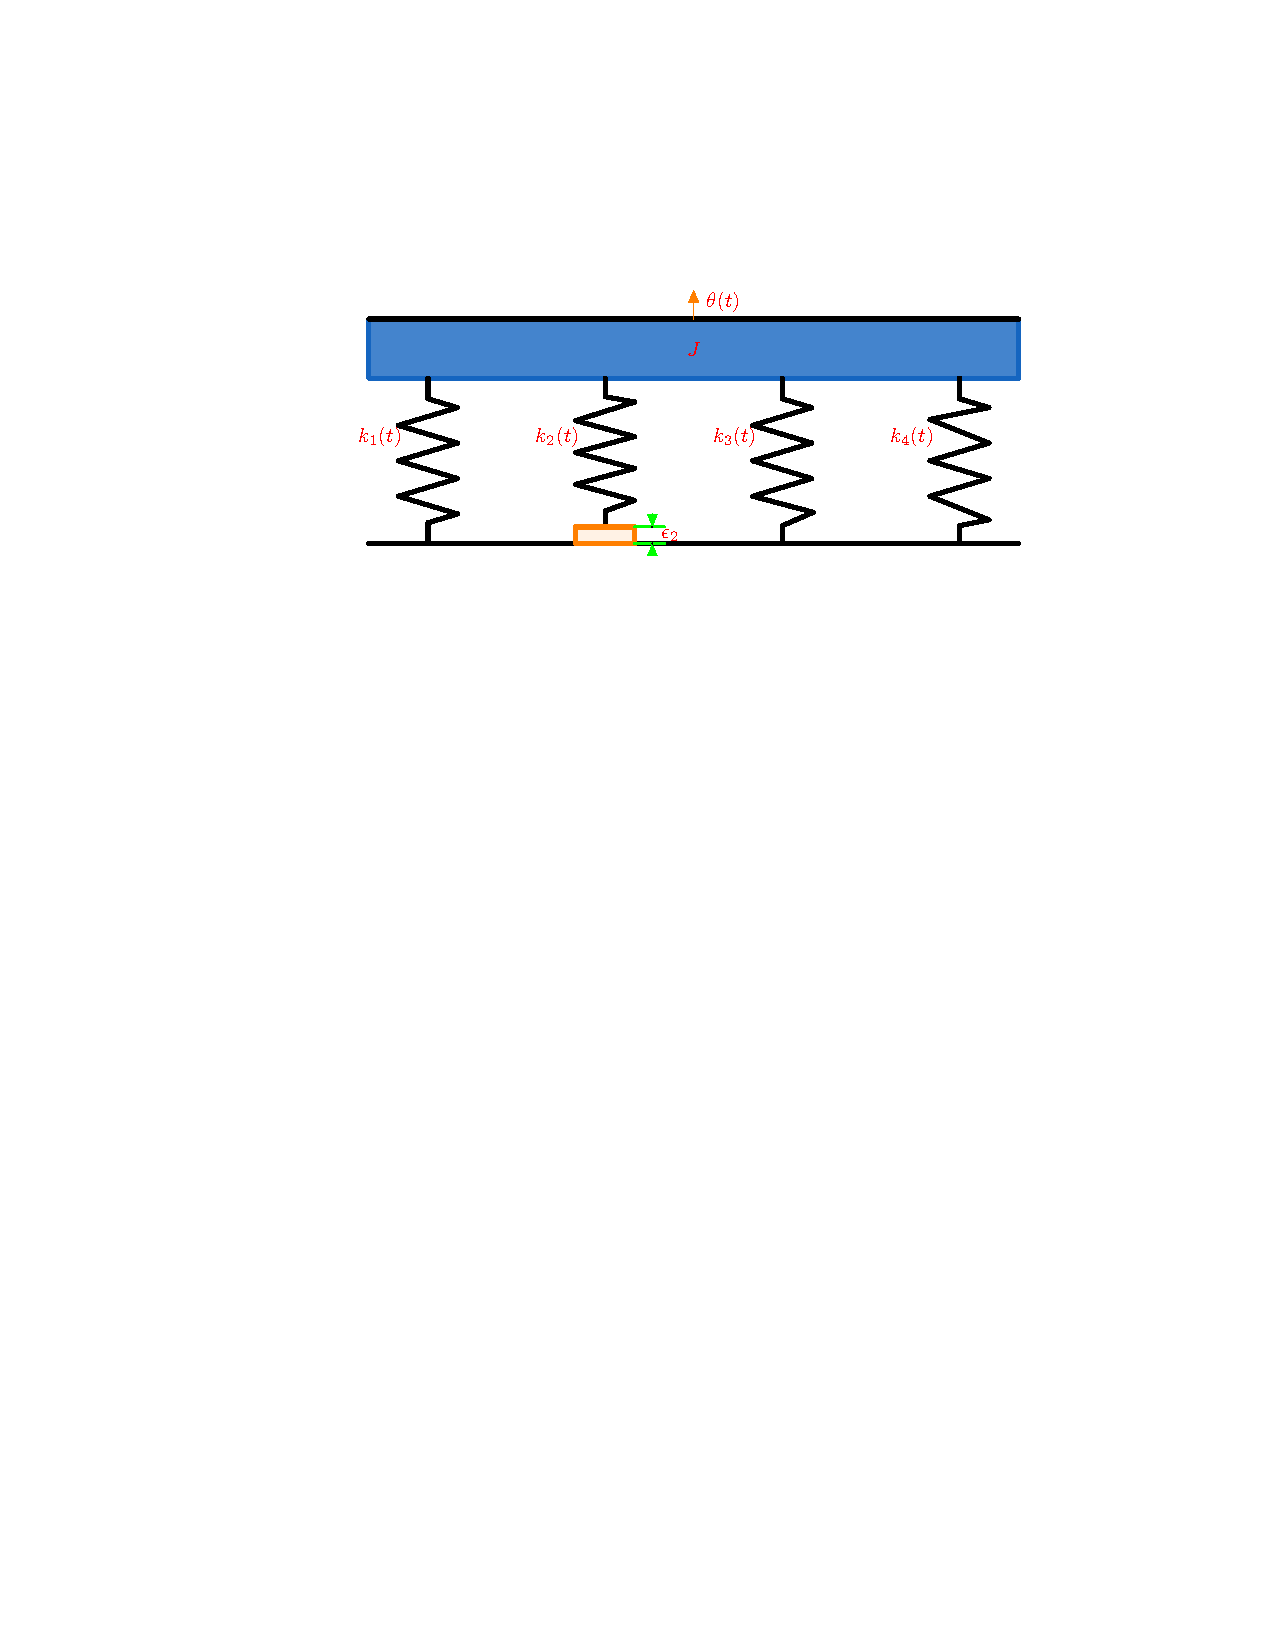
\includegraphics[scale=0.6,width=0.8\textwidth,height=1.6in]{spring_mass.pdf}
        \caption{Vibration system of unequal load sharing among four planets.}
    \label{fig:vibration_system_of_spring_mass}
    \end{figure*}
\end{enumerate}

\subsection{Planetary gearbox structure}
\par A typical layout of planetary gearboxes consists of three kinds of gears mounted so that the centers of planet gears revolves around the center of sun and ring gears, as shown in Fig. \ref{fig:planetary_gearbox_layout}. This paper merely discusses the common cases of speed reducers where the sun gear connects with the power input shaft and the carrier works as power output, while vibration sensors are usually mounted on the surface of the stationary ring gear in diagnostic applications. 
\begin{figure}[pos=htbp]
    \centering
    \begin{annotate}{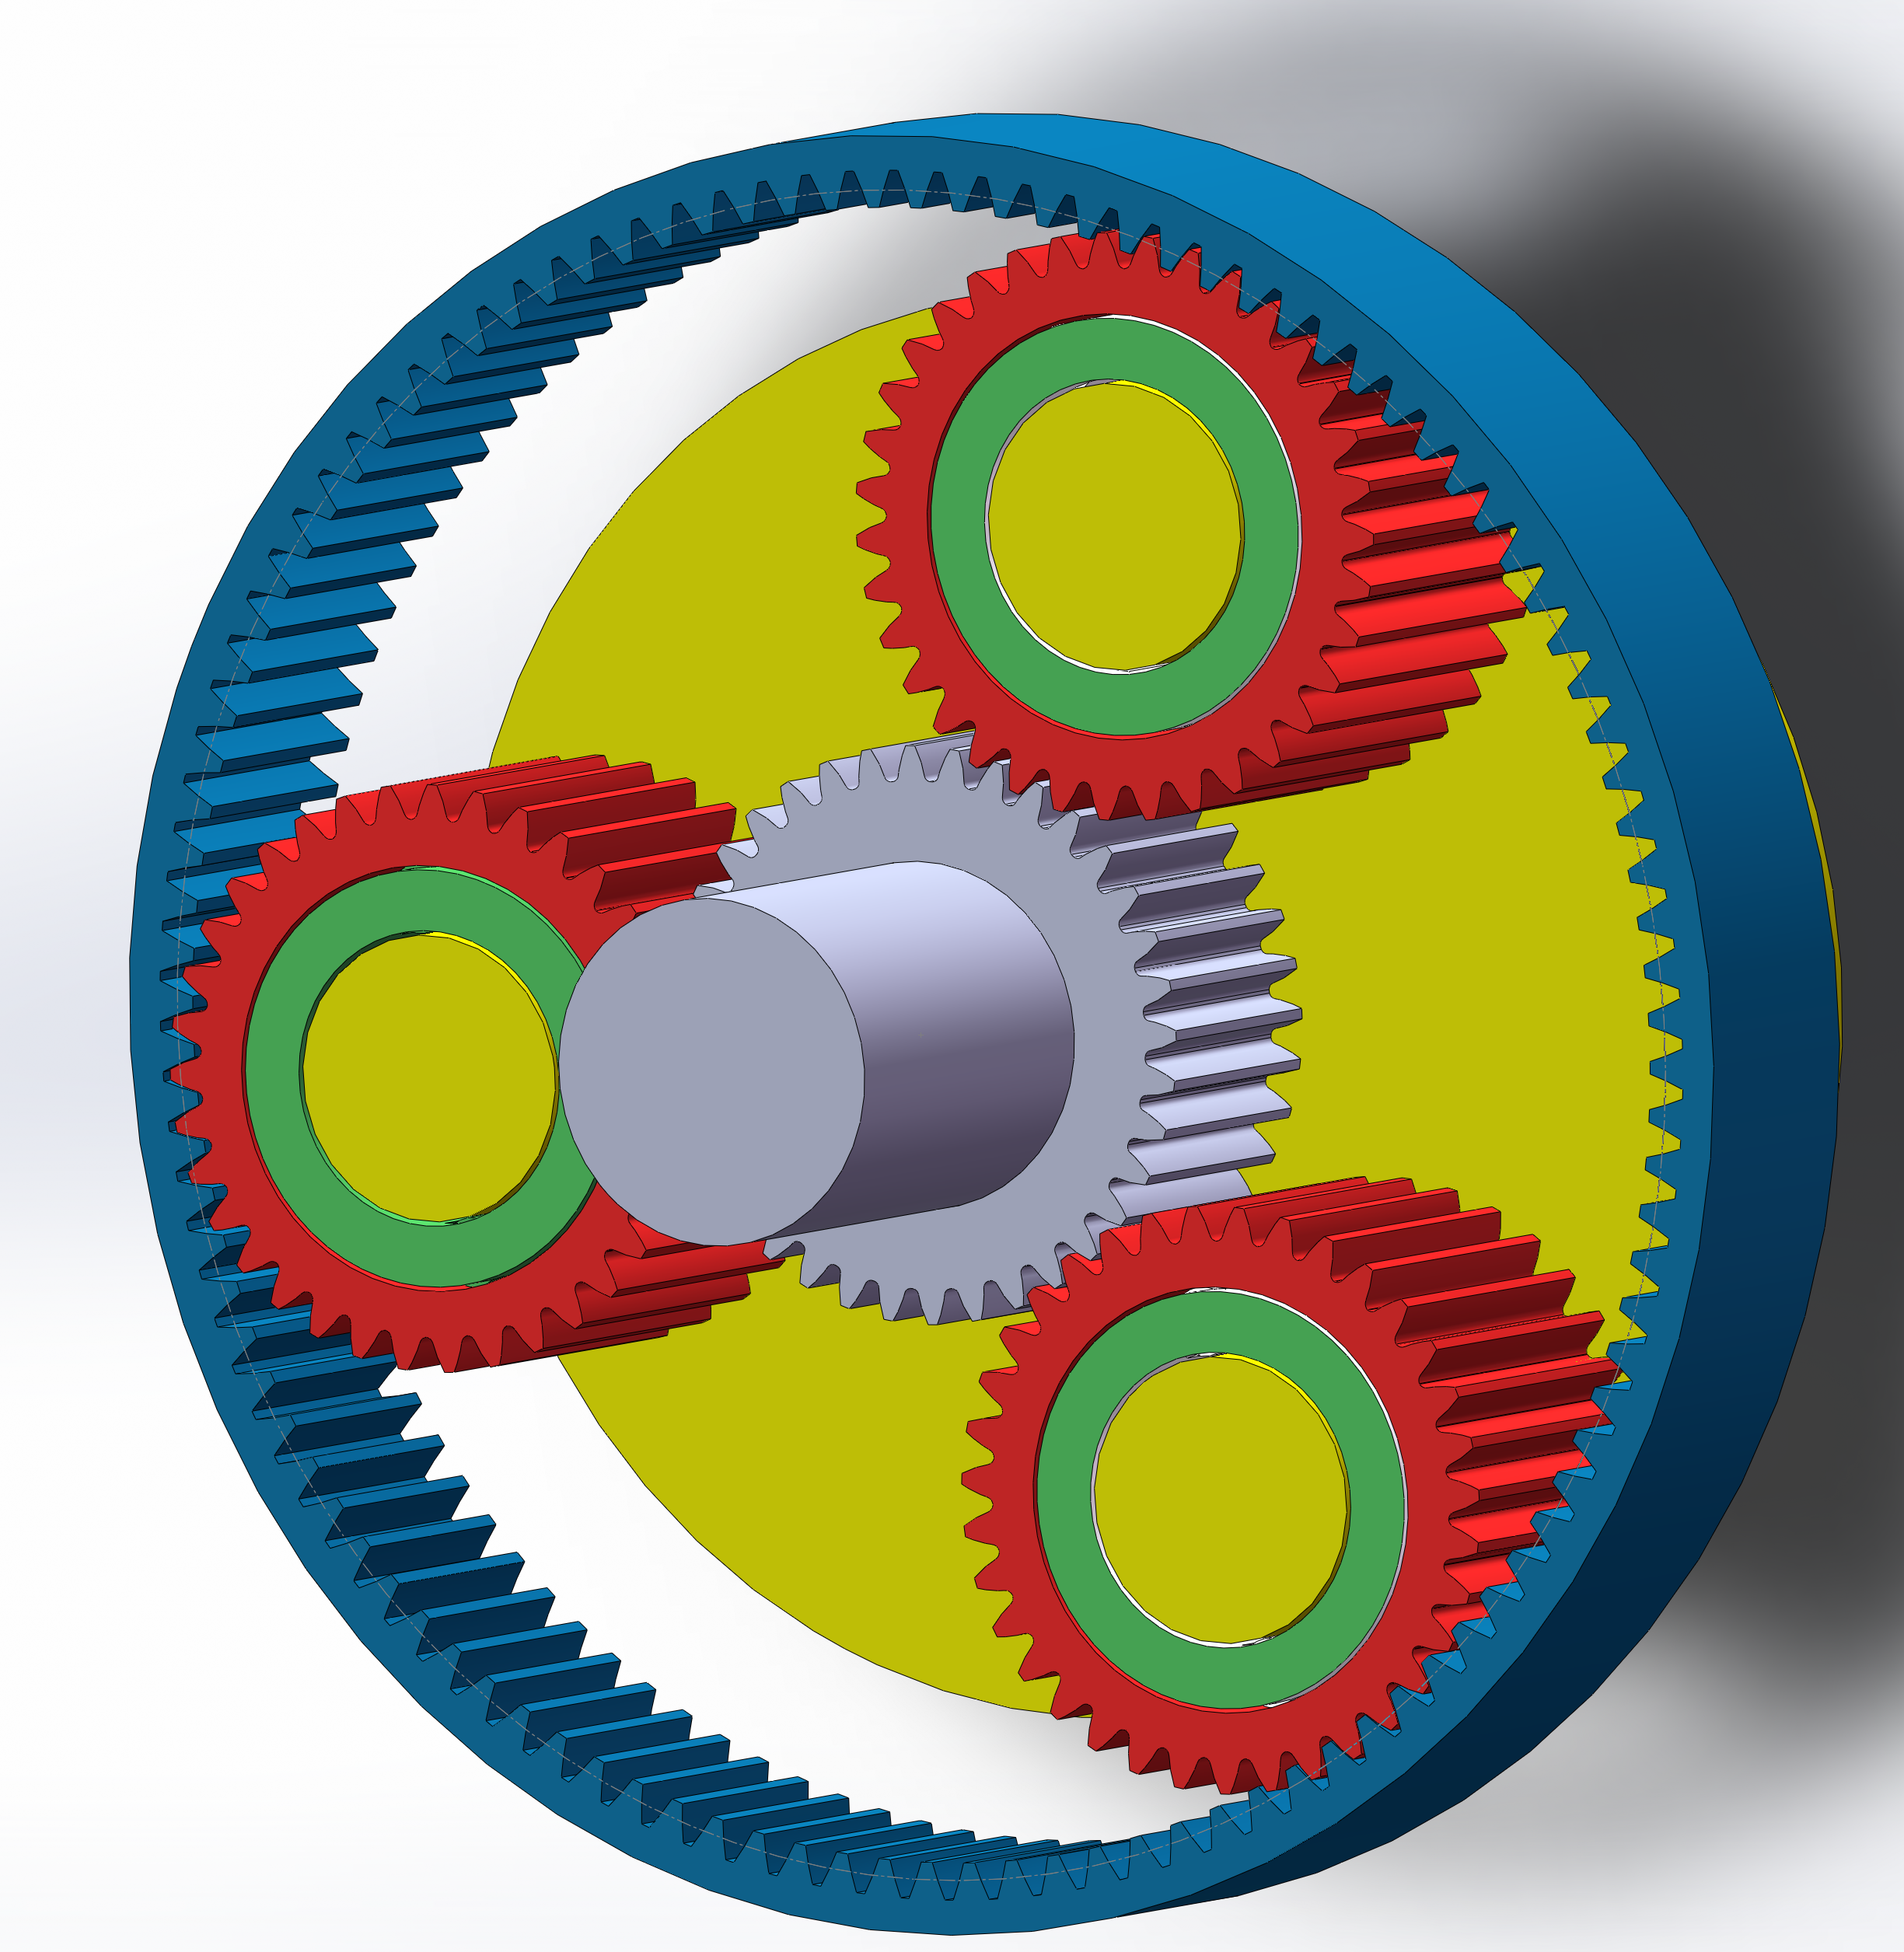
\includegraphics[width=0.3\textwidth]{Planetary_Gearbox.PNG}}{0.3}
        \callout{-8,-7}{Ring gear}{-5,-5.8}
        \callout{8,-7}{Planet gear}{4,-5.5}
        \callout{-8,7}{Sun gear}{-0.8,1.2}
        \callout{8,7}{Carrier}{4.5,1}
    \end{annotate}
    \caption{Configuration of planetary gearboxes.}
    \label{fig:planetary_gearbox_layout}
\end{figure}
\par The vibration in planetary gearboxes mainly origins from the meshing of gears \cite{Velex1996}. When the planet gears engage with the ring gear or sun gear, the number of the involved tooth varies with the relative rotation between gears and their contact stiffness changes consequently. The transmission load nominally remains constant and the gearbox is a parametrically excited multi-degree-freedom system \cite{Acar2019}. 
\subsection{Vibration of single planet}
\par To figure out the vibration mechanism of planetary gearboxes, we start with the meshing vibration of a pair of gears. For an individual planet, the vibration model can be written as
\begin{equation}
    J \cdot \ddot{\theta}(t) + k(t) \cdot \theta(t) = 0 \label{eq:1_DOF_vibration},
\end{equation}
where \(J\) is rotational inertia of the machine, \(\theta(t)\) is the shaft angular, \(\ddot{\theta}(t)\) is the rotational acceleration, \(k(t)\) is time-varying meshing stiffness and fluctuates in the form
\begin{equation}
    k(t)=k_0+2 q \cos(2 \pi f_{\rm m} t) \label{eq:meshing_stiffness},
\end{equation}
where \(k_0\) is the nominal meshing frequency, \(q\) denotes the the fluctuation intensity, and \(f_{\rm m}\) is the meshing frequency. Substitute Eq. (\ref{eq:meshing_stiffness}) into the Eq. (\ref{eq:1_DOF_vibration}), we have
\begin{equation}
    J \cdot \ddot{\theta}(t) + \left[k_0+2 q \cos(2 \pi f_{\rm m} t)\right] \cdot \theta(t) = 0. \label{eq:mathieu_function}
\end{equation}
\par Eq. (\ref{eq:mathieu_function}) is the Mathieu function. According to the Floquet theory \cite{Arscott2014}, its general solution the product of an exponential part and a harmonic part. Taking damper into account, we only consider stable operation conditions so that harmonic solution is concentrated. The response of the model in Eq. (\ref{eq:mathieu_function}) has the same harmonic component \(\cos(2 \pi f_{\rm m} t)\). In the situation where the time-varying meshing stiffness of all planets are considered, the solution has the corresponding harmonic components (at the same frequency \(f_{\rm m}\) with different phases in planetary gearboxes).
The oscillation of gear meshing stiffness primarily contributes the vibration of planetary gearboxes.
\subsection{General signal model}
\par The signal model perceived by the stationary transducer on the gearbox housing can be modelled as the summation of all planet vibration considering transfer path effects. The impulsive intensity of gear meshing is assumed to proportional to the load applied on each planet. The vibration of each planet is divided into planet-ring and planet-sun parts. Thus, the general signal model is
\begin{equation}
    x(t)=\sum_{i=1}^{M} L_i \cdot \left[ \sigma_{{\rm r}i}(t) \xi_{{\rm r}i}(t) + \sigma_{{\rm s}i}(t) \xi_{{\rm s}i}(t) \right], \label{eq:general_signal}
\end{equation}
where $M$ is the planet number, $L_i$ denotes the load sharing coefficient, $\sigma_{\rm pr}$ and $\sigma_{\rm ps}$ denotes transfer path effect on planet-ring and planet-sun gears, respectively, $\xi_{{\rm r}i}$ and $\xi_{{\rm s}i}$ are the vibration originating from the $i$-th planet-ring and planet-sun gears.
\par Nominally, all planet center distribute along circumference of the carrier evenly. Without loss of generality, the nominal angular position of first planet center is set as zero, and
\begin{equation}
    \Theta_i=\frac{(i-1)\cdot 2\pi}{M},
\end{equation}
where $\Theta_i$ denotes the nominal position of $i$-th planet. In addition, due to the manufacturing or assembling process, each planet center deviates from the nominal position by $\epsilon_i$. If $\epsilon_i>0$, the planet engages with the ring or sun gear in advance, or negative error represents the engagement lag. We can assume $\epsilon_1=0$ in the coordinate system, because these planets locate relatively to each other. Even if $\epsilon_1 \neq 0$, we can also set $\epsilon_i=\epsilon'_i-\epsilon'_1,i \geq 2$, where $\epsilon'_i$ is $i$-th planet error in another coordinate system.
\par To reveal the spectral structure simply, the gear meshing vibration of each planet is regarded as Dirac comb function $\operatorname{III}(t)=\sum_{i=-\infty}^{+\infty}\delta(t-i)$. The meshing frequency can be calculated by different engaging gears,
\begin{equation}
    f_{\rm m}=Z_{\rm r} \cdot (f_{\rm r}+f_{\rm c})=Z_{\rm p} \cdot (f_{\rm p}-f_{\rm c})=Z_{\rm s} \cdot (f_{\rm s}-f_{\rm c}). \label{eq:meshing_frequency}
\end{equation}
where $\{\}_{\rm r}$, $\{\}_{\rm p}$, $\{\}_{\rm s}$, $\{\}_{\rm c}$ denote ring gear, planet, sun gears and carrier, respectively; $Z_{\{\}}$ is the gear number and $f_{\{\}}$ is the rotating frequency. 
\par For planet-ring gears, the planet angular position error bring about the time shift. The time shift is the angular error divided by the relatively rotating velocity. Thus, the planet-ring meshing vibration can be written as
\begin{equation}
    \xi_{{\rm r}i}(t)=A_{{\rm r}i}\operatorname{III}\left[f_{\rm m} \cdot (t-\frac{\epsilon_i+\Theta_i}{2 \pi f_{\rm c}})\right],\label{eq:planet-ring_meshing}
\end{equation}
where $A_{{\rm r}i}$ is the impulsive amplitude of $i$-th planet-ring gear meshing, the $f_{\rm m}$ is the meshing frequency. Park et al. propose the difference between planet-ring and planet-sun meshing phase \cite{Parker2004}. Similarly, the planet-sun meshing vibration is
\begin{equation}
    \xi_{{\rm s}i}(t)=A_{{\rm s}i} \operatorname{III}\left[f_{\rm m} \cdot (t + \frac{\epsilon_i+\Theta_i}{2 \pi f_{\rm s}- 2 \pi f_{\rm c}})+ \frac{\varphi_i}{2 \pi} \right],\label{eq:planet-sun_meshing}
\end{equation}
where $A_{{\rm r}i}$ is the impulsive amplitude of $i$-th planet-sun gear meshing, $\varphi_i$ is the phase difference between planet-ring and planet-sun meshing for the $i$-th planet.
\subsection{Unequal load sharing among planets (Add the 5 and 6 planet cases)}
\par The multiple paralleled power paths formed by planets can sharing torque load. This merit of planetary gearboxes will compromise when the load sharing inequality occurs. The position errors of planet pinholes or bearings in the tangential (circumferential) direction happening in manufacturing and assembling lead to the non-uniform loads on planets \cite{Singh2010511-530}. In this section, we assume the load is heavy and the pinhole position errors are small, so that all planets are loaded. To partly centralize the uneven load, planetary gearboxes usually permit at least one floating central member (sun gear or carrier). The formula of load sharing ratio of a 4-planet planetary gearbox as follows \cite{Ligata2009}
\begin{equation}
    L_i=\frac{1}{4}+\frac{k_{\rm e} r_{\rm s}}{8 T_{\rm s}}\left(e_i-e_{i+1}+e_{i+2}-e_{i+3}\right), i=1,2,3,4. \label{eq:load_sharing_ratio}
\end{equation}
In this formula, \(L_i\) denotes the load sharing ratio of the \(i\)-th planet, \(k_{\rm e}\) is the effective support stiffness concerning both the bearing and gear meshing and described in Eq. (\ref{eq:stiffness}), \(r_{\rm s}\) is the sun gear pitch radius, \(T_{\rm s}\) is the total torque applied on input sun gear. For any \(i>4\) in Eq. (\ref{eq:load_sharing_ratio}), \(i=i-4\). The tangential error $_{i}$ can be calculated by Eq. (\ref{eq:tangential_error}).
In this formula, \(L_i\) denotes the load sharing ratio of the \(i\)-th planet, \(k_{\rm e}\) is the effective support stiffness concerning both the bearing and gear meshing and described in Eq. (\ref{eq:stiffness}), \(r_{\rm s}\) is the sun gear pitch radius, \(T_{\rm s}\) is the total torque applied on input sun gear. For any \(i>4\) in Eq. (\ref{eq:load_sharing_ratio}), \(i=i-4\). The tangential error $\epsilon_{i}$ can be calculated by Eq. (\ref{eq:tangential_error}) and its explanation see Fig. \ref{eq:tangential_error}.
\begin{equation}
    k_{\rm e}=\frac{1}{k_{\rm rp}+k_{\rm sp}}+\frac{1}{k_{\rm b}},\label{eq:stiffness}
\end{equation}
where $k_{\rm rp}$ and $k_{\rm sp}$ are the meshing stiffness of planet-ring and planet-sun, respectively, $k_{\rm b}$ is the planet bearing stiffness.
\begin{equation}
    e_{i}=2(R_{\rm r}-R_{\rm p})\sin(\epsilon_{i}/2)\cos(\epsilon_{i}/2),\label{eq:tangential_error}
\end{equation}
where $R_{\rm p}$ is the planet radius, $R_{\rm s}$ is the sun radius, $\epsilon_{i}$ is the angular position error the $i$-th planet.
\begin{figure}[pos=htbp]
    \centering
    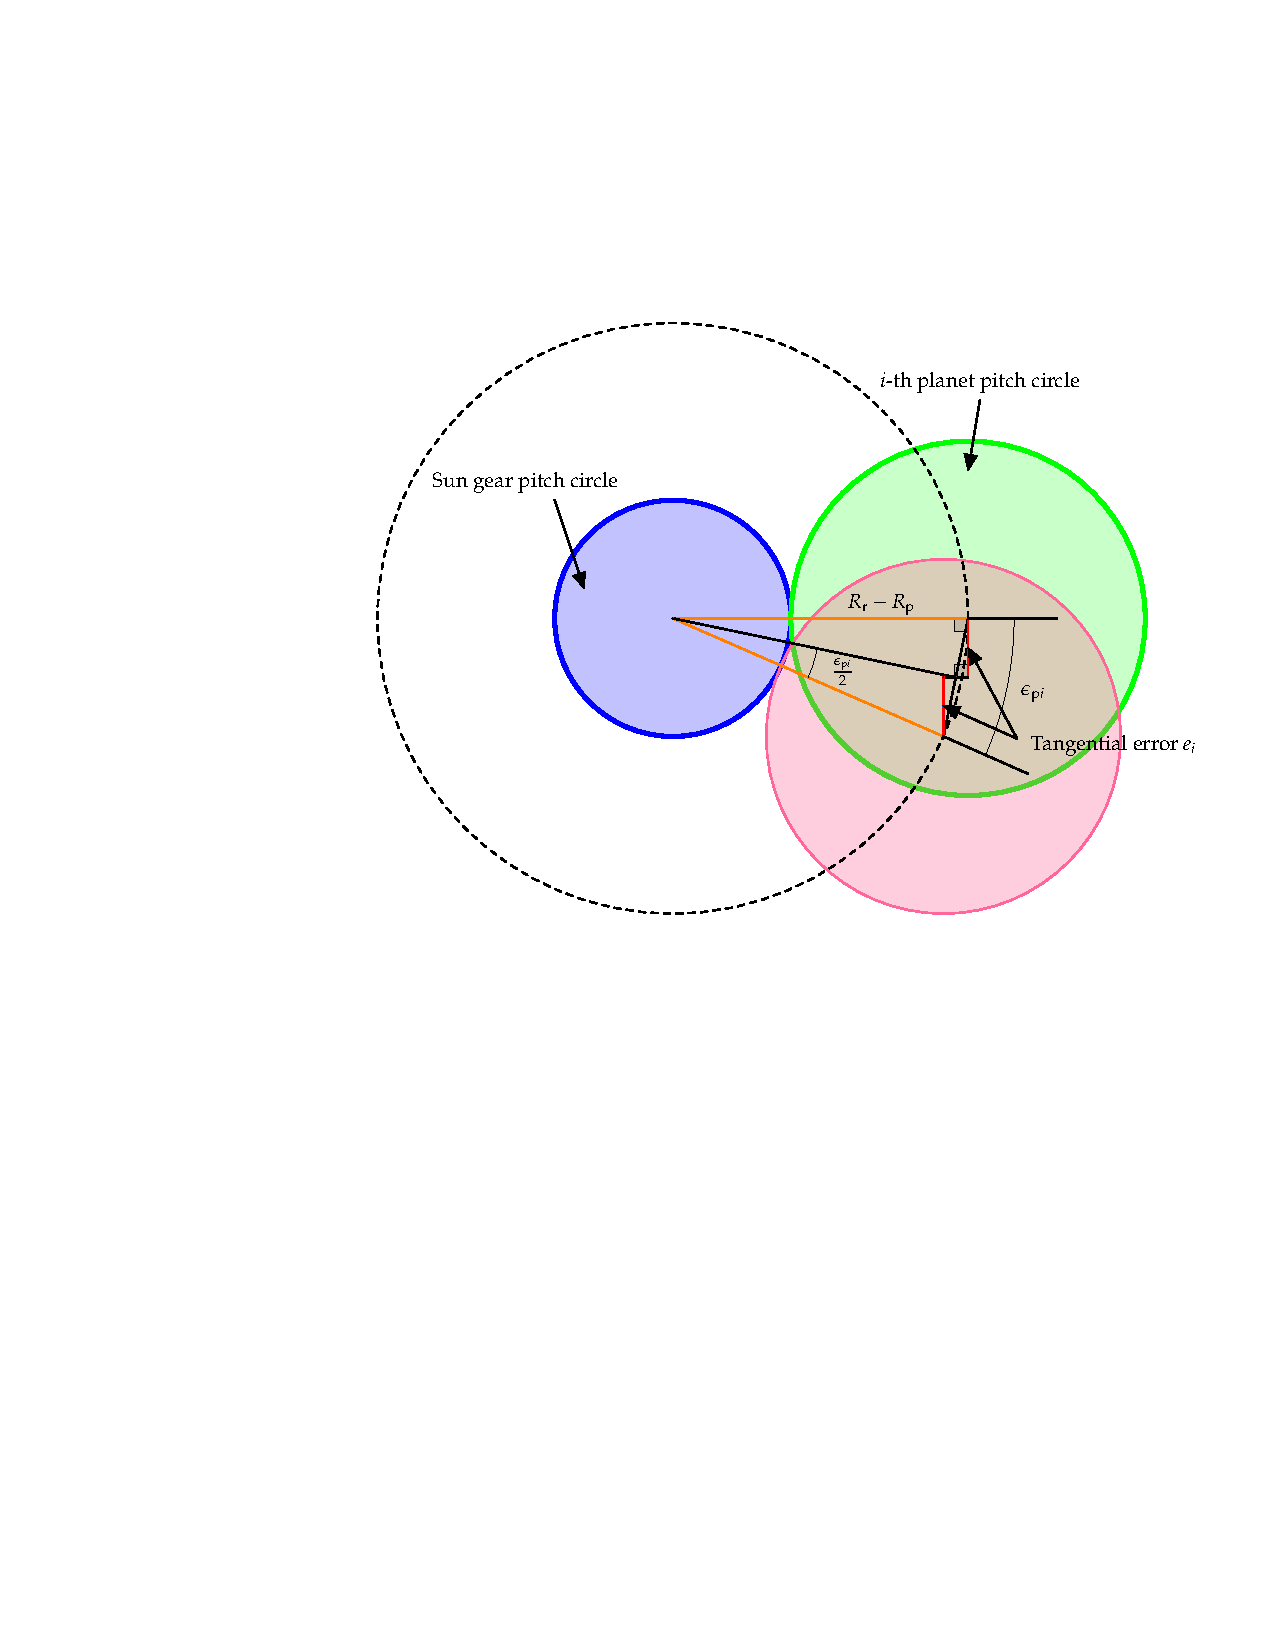
\includegraphics[scale=0.5]{tangential_error.pdf}
    \caption{Tangential error calculation (correct the $\epsilon_{pi}$)}
    \label{fig:tangential_error}
\end{figure}
\par Unequal load sharing will gives rise to non-uniform impulsive intensity. The acceleration are linearly affected by the dynamic force exerted. Thus, the vibration amplitude of each planet is assumed to be proportional to the load applied on it \cite{Inalpolat2009}. In other words, planet load modifies the amplitude of the vibration signal. Moreover, the unevenly planet distribution along the angular position of carrier also has phase modulation when the transfer path is considered simultaneously. These effects will be illustrated explicitly in the later discussion. 
\subsection{Transfer paths}
\par The vibration originating from the planet meshing with ring or sun gear propagate through several paths to the stationary sensor mounted on the case. As demonstrated in Fig. \ref{fig:transfer_path}, there are three paths for planet-ring and planet-sun gear meshing, respectively. These transfer paths can be categorized into two types, depending on whether or not they pass through bearings. The paths passing through bearings (path 2, 3, 5, 6 in Fig. \ref{fig:transfer_path}) must transfer via the gearbox housing to reach the sensor fixed on the top. Compared with the paths merely passing through gears (path 1, 4 in Fig. \ref{fig:transfer_path}), these paths passing bearings are longer and more likely to be attenuated by the lubricating oil layer in bearings \cite{Feng2012}. To simplify modelling, only the shorter paths (path 1, 4 in Fig. \ref{fig:transfer_path}) are concerned in this paper.
\begin{figure}[pos=htbp]
    \centering
    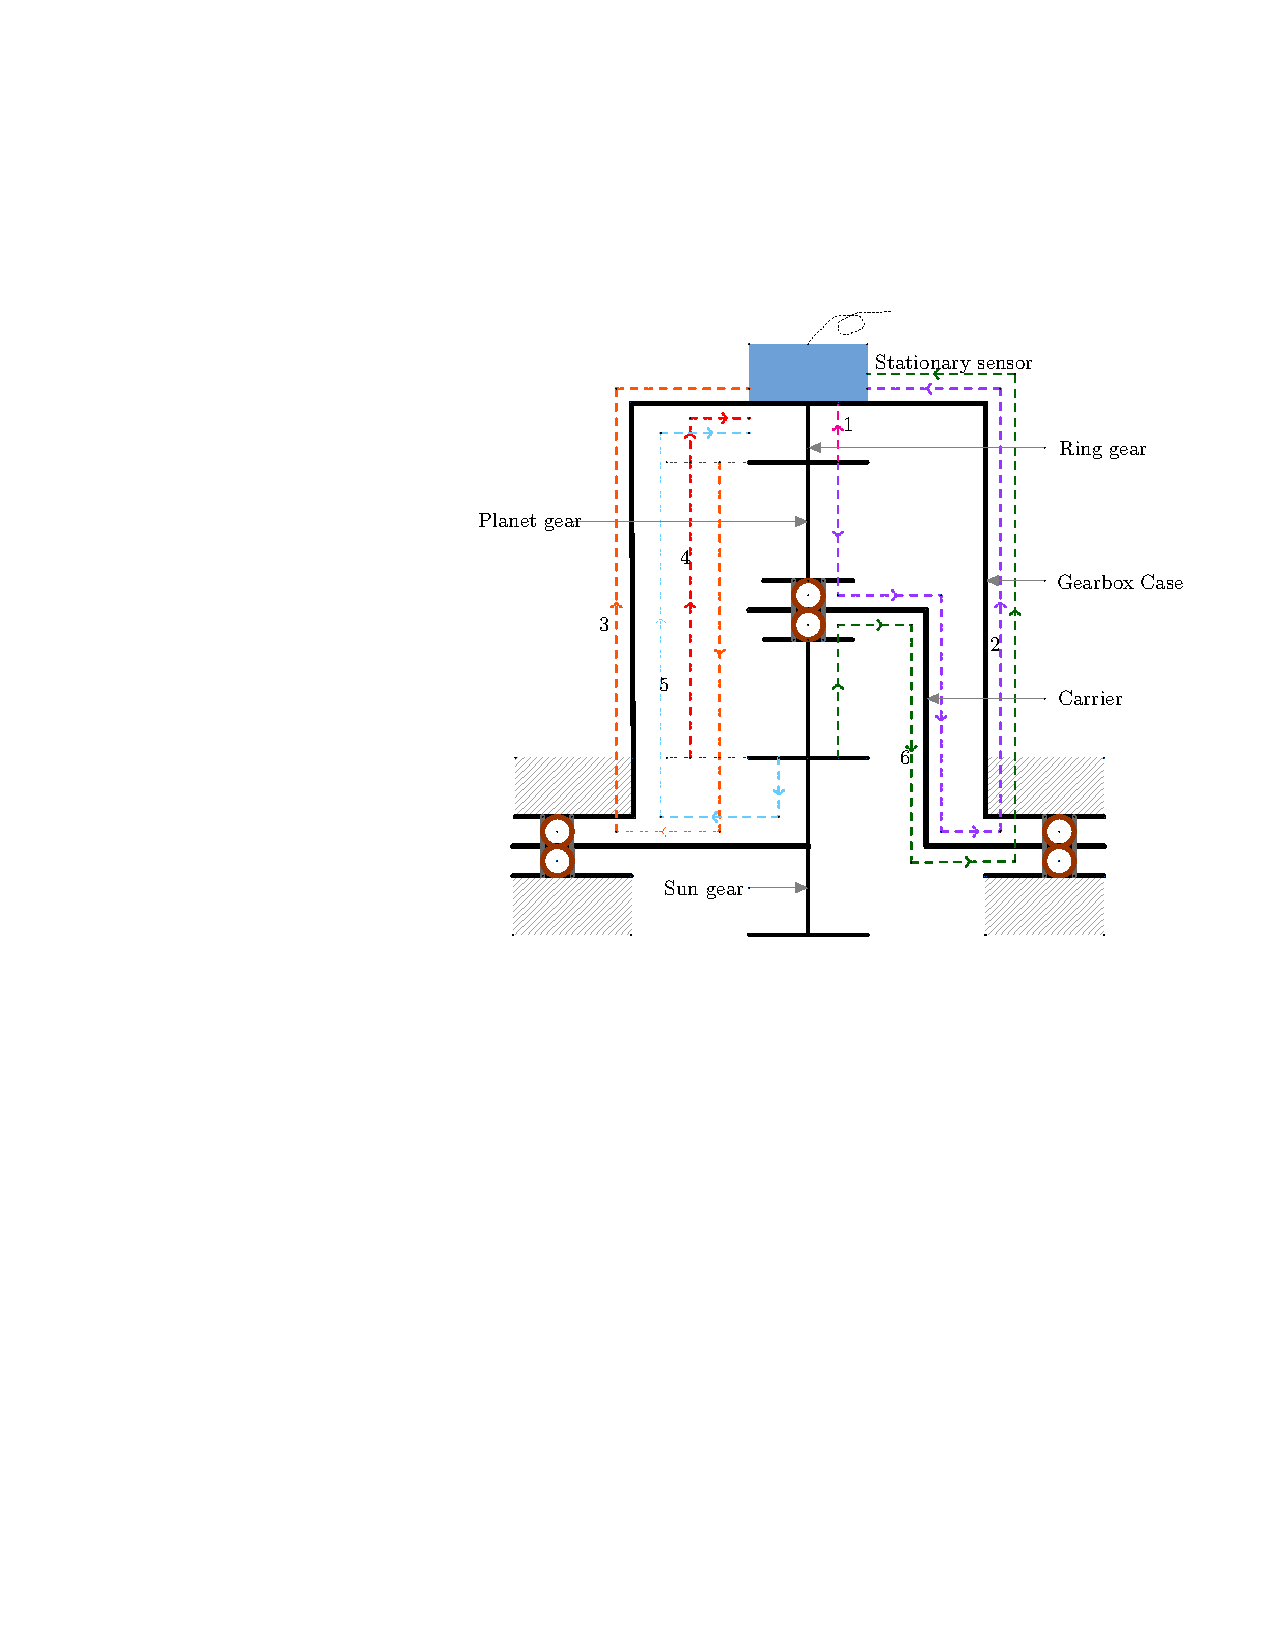
\includegraphics[scale=0.5]{transfer_path.pdf}
    \caption{Transfer paths of gear meshing vibration.\textbf{add explanation on path number. from where to where.}\label{fig:transfer_path}}
\end{figure}
\par The lengths of path 1 and path 4 vary with the circumferential position of carrier. For each planet, the meshing vibration points get close to the fixed sensor as the planet approaches the top surface of gearbox case. When the planet reach the climax of its revolution circle, the fixed transducer percepts the maximum impulsive strength. While the planet arrives at the case bottom, the perceived impulses are most weakened. The path 1 length is triangle wave of time (as shown in Fig. \ref{fig:path_length_trangle_wave}) when planetary gearboxes operate at a constant speed and planet distributes evenly, 
\begin{equation}
    l_{{\rm r}i}(t)=
    \begin{cases}
        2 \pi R_{\rm r} f_{\rm c} \left|t-(\frac{\epsilon_i+\Theta_i}{2 \pi f_{\rm c}} + \frac{n}{f_{\rm c}}) \right|, \frac{n}{f_{\rm c}} - \frac{1}{2 M f_{\rm c}} + \frac{\epsilon_i+\Theta_i}{2\pi  f_{\rm c}} \leq t < \frac{n}{f_{\rm c}} + \frac{1}{2 M f_{\rm c}} + \frac{\epsilon_i+\Theta_i}{2\pi f_{\rm c}}, n\in \mathbb{Z} , i=1,2,\ldots,M\\
        +\infty, \quad \text{otherwise}
    \end{cases},
\end{equation}
where $M$ is the planet number. The path 4 is the sum of the diameter of the planet pitch circle and $l_{{\rm r}i}$,
\begin{equation}
    l_{{\rm s}i}(t)=l_{{\rm r}i}+2 R_{\rm p}. \label{eq:path_4_length}
\end{equation}
\begin{figure}[pos=htbp]
    \centering
    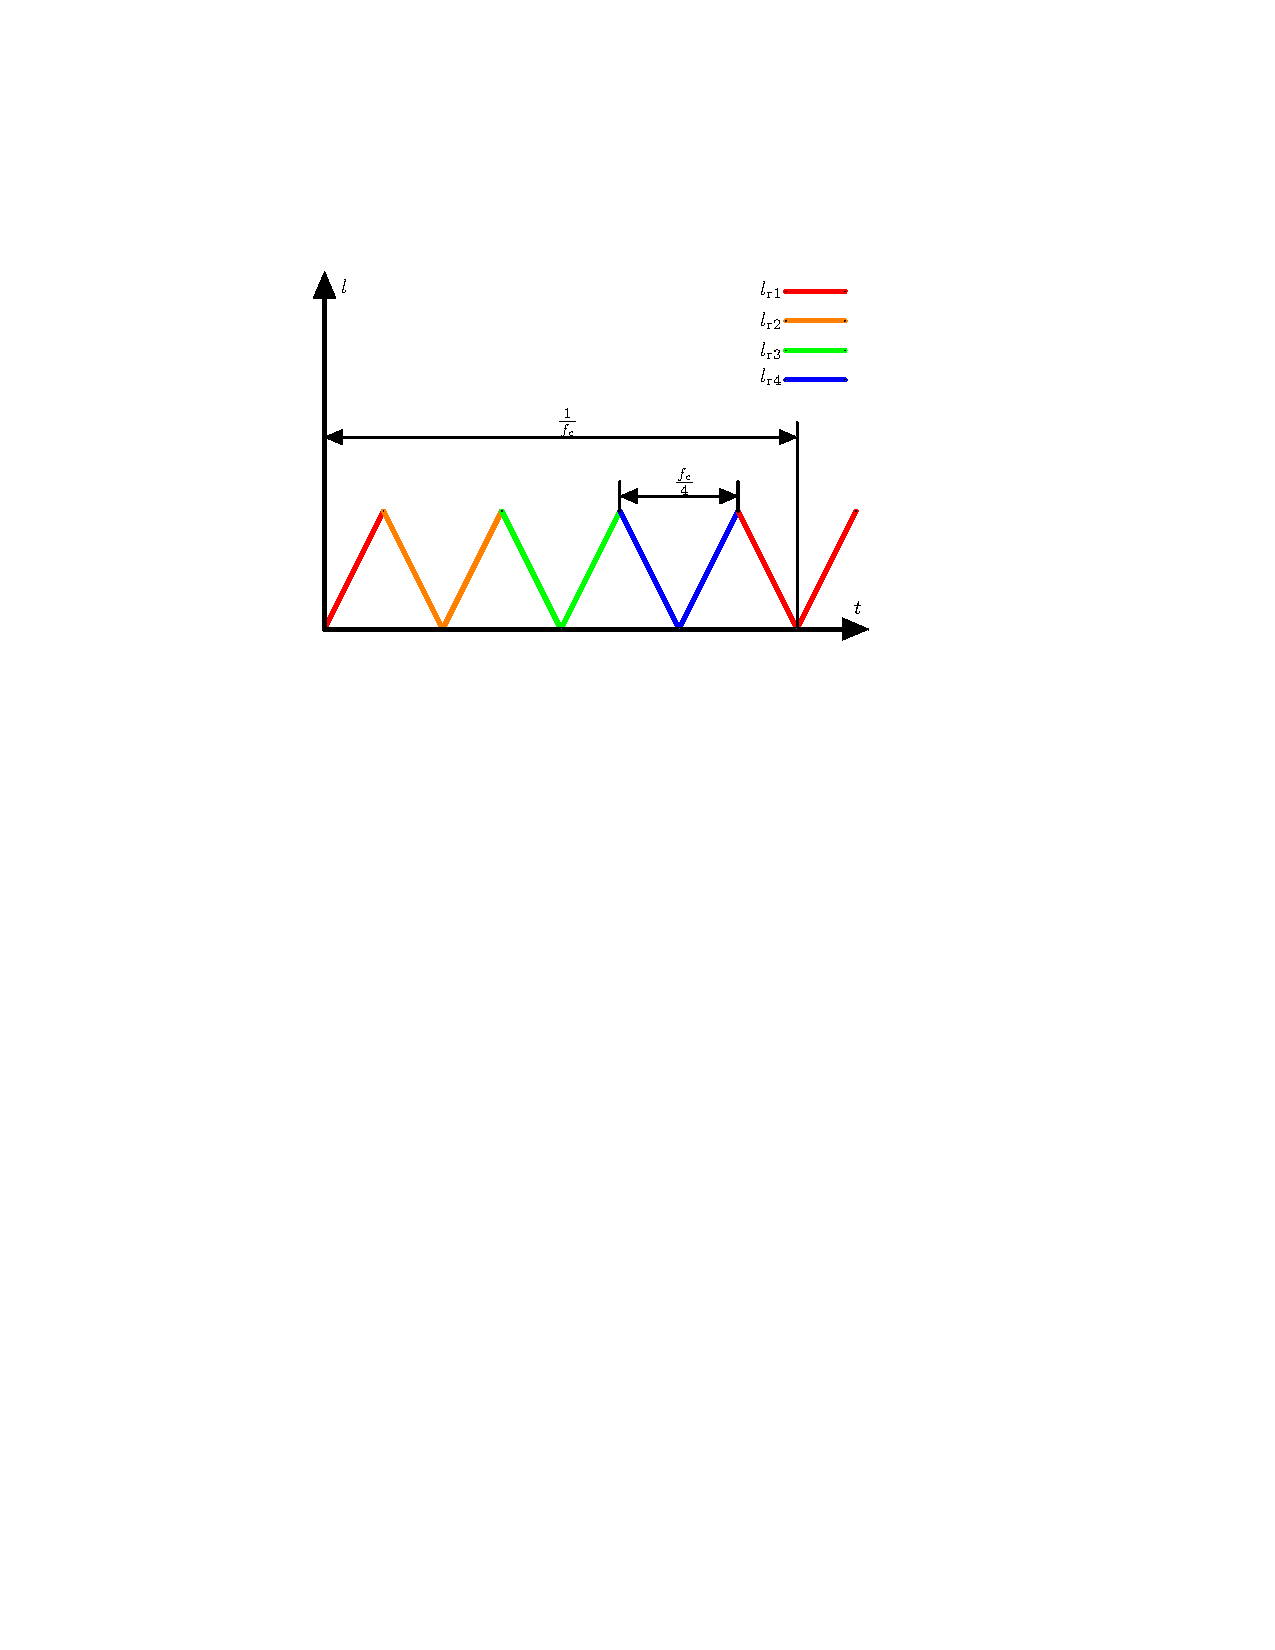
\includegraphics[scale=0.5]{trangle_wave.pdf}
    \caption{Transfer Path 1 length function of time. \textbf{vary the line type for different lengends.Add the transfer effect funciton of time}}
    \label{fig:path_length_trangle_wave}
\end{figure}
\par This attenuation effect with regard to the path length can be characterized as window functions such as Hanning window or Gaussian window \cite{Mark2009}. In this paper, we apply the Gaussian window describing the time-varying transfer path effect,
\begin{equation}
    \sigma(l)=F\exp\left(-\frac{l}{a}\right),\label{eq:general_transfer_path}
\end{equation}
where $l$ is the length of a transfer path, $F$ represents for the strength factor and $a$ is the attenuation factor. The larger $a$ is, the longer impulses can propagate without a large energy loss. Given Eq. (\ref{eq:path_4_length}) and Eq. (\ref{eq:general_transfer_path}), we can deduce the proportional relationship between path 1 and path 4,
\begin{equation}
    \sigma (l_{{\rm s}i})=F\exp(-\frac{l_{{\rm r}i}+2 R_{\rm p}}{a})=\exp(-\frac{2 R_{\rm p}}{a}) \cdot \sigma(l_{{\rm r}i}).
\end{equation}
For simplicity, we set the $\sigma_i(t)=\sigma\left[l_{{\rm r}i}(t)\right]$ and $\eta=\exp(-\frac{2 R_{\rm p}}{a})$. Fig. \ref{fig:path_length_trangle_wave} shows that $\sigma_{i}(t)$ shifts in time by $(\epsilon_i-\Theta_i)/(2 \pi f_{\rm c})$ relative to $\sigma_1$:
\begin{equation}
    \sigma_{i}(t)=\sigma_{1}(t-\frac{\epsilon_i+\Theta_i}{2 \pi f_{\rm c}}).
\end{equation}
\par Because the transfer path effect function is the exponential function shifting along the time axis with a fixed interval, it can be rewritten as the convolution of exponential function and Dirac comb function with the carrier rotation period $1/f_{\rm c}$.
\begin{equation}
    \sigma_i(t)=\sigma_0(t) \ast \operatorname{III}\left[f_{\rm c} (t - \frac{\epsilon_i+\Theta_i}{2 \pi f_{\rm c}})\right],\label{eq:transfer_path_convolution_form}
\end{equation}
where
\begin{equation}
    \sigma_0(t)=\begin{cases}F \exp(\frac{- 2 \pi R_{\rm r} f_{\rm c} \left|t\right|}{a}),\quad &\frac{-1}{2 M f_{\rm c}} \leq t < \frac{1}{2 M f_{\rm c}}\\
        0, &\text{otherwise}.
    \end{cases}\label{eq:tranfer_path_time_shape}
\end{equation}
\subsection{Natural frequency\labe{sec:natural_frequency}}
\par In the above discussion, the gear meshing vibration is simply considered as Dirac impulses. In practice, every impact arising from different components will excite the machine natural frequency. The excited resonance affects the spectral structure globally: the amplitudes of the vibration frequencies around the natural frequency are reinforced and other amplitudes are attenuated. The resonance features a harmonic wave with the amplitude attenuating exponentially, like the vibration of a spring-mass-damper,
\begin{equation}
    \lambda(t)=\begin{cases}
        \exp(-t/\beta)\cdot \sin(2 \pi f_{\rm n} t),\quad & t>=0\\
        0, & t<0
    \end{cases},
\end{equation}
where $\beta>0$ is the structural damping coefficient, $f_{\rm n}$ is the natural frequency.
\par Every time a gear meshing vibration occurs, the machine's natural vibration is excited. This process is mathematically equivalent to the convolution of the impact function of the meshing vibration with the exponentially attenuated harmonic function of the natural vibration. Therefore, considering the effect of the natural vibration, the above signal model can be updated into
\begin{equation}
    \widetilde{x} (t)=\lambda(t) \ast \sum_{i=1}^{M} L_i \sigma_i(t) \left\{ \operatorname{III}\left[f_{\rm m} \cdot (t-\frac{\epsilon_i+\Theta_i}{2 \pi f_{\rm c}})\right]% planet-ring part
    + \eta \operatorname{III}\left[f_{\rm m} \cdot (t + \frac{\epsilon_i+\Theta_i}{2 \pi f_{\rm s}-2 \pi f_{\rm c}}) + \frac{\varphi_i}{2 \pi} \right]% planet-sun part
    \right\},\label{eq:final_signal_model}
\end{equation}
where $\ast$ denotes convolution.
\par For machines with the same configuration, when the load distribution of the planet is uneven, the contact stiffness of the transfer path of each planet inside the planetary gearbox will decrease relative to the case of the uniform load distribution. As a result, The decrease of internal contact stiffness will lead to the decrease of natural frequency of the whole system. Therefore, the variation of the system's natural frequency can be used as a circumstantial evidence to diagnose the load distribution among planets.
\par If the planet pinhole distribute evenly on the carrier, the number of the planets bearing the input load varies as the applied load increases gradually. When the load starts at almost zero, only three planets or one pair of diagonal planets simultaneously engaging with sun and ring gear \cite{Ligata2009}. In this circumstance, load sharing coefficients $L_i=0$ for the unloaded planets. With the ascending input load, another pair of gears get involved. At the same time, the entire transmission system stiffen because more gears support the connection between the input and output. The natural frequency rises along with the system stiffness because the natural frequency equals the square root of stiffness over mass.
\section{Spectral structure}
\par In this section, we will derive the spectral structure of the above proposed signal model for the in-depth understanding of planetary gearbox vibration. Because natural vibration merely affects the spectral envelope shape, we can consider it separately later on. The gear meshing vibration (Eq. (\ref{eq:planet-ring_meshing}) and Eq. (\ref{eq:planet-sun_meshing})) and transfer path effect arising from the carrier rotation $\sigma_{i}(t)$ are periodic with periods $1/f_{\rm m}$ and $1/f_{\rm c}$, respectively. According to Eq. (\ref{eq:meshing_frequency}) and $f_{\rm r}=0$, $f_{\rm m}=Z_{r} \cdot f_{\rm c}$. Apply Fourier transform to the planet-ring vibration, yields
\begin{equation}
\begin{split}
    \mathcal{F}\left[ \sigma_{{\rm r}i}(t) \xi_{{\rm r}i}(t) \right]=&\mathcal{F}\left\{\sigma_0(t) \ast \operatorname{III}\left[f_{\rm c} \cdot (t - \frac{\epsilon_i+\Theta_i}{2 \pi f_{\rm c}})\right] \cdot A_{{\rm r}i}\operatorname{III}\left[f_{\rm m} \cdot (t-\frac{\epsilon_i+\Theta_i}{2 \pi f_{\rm c}})\right]\right\}\\
    =&A_{{\rm r}i} \cdot \mathcal{F}\left[\sigma_0(t)\right] \cdot \mathcal{F}\left\{\operatorname{III}\left[f_{\rm c} \cdot (t - \frac{\epsilon_i+\Theta_i}{2 \pi f_{\rm c}})\right] \right\}
    \ast \mathcal{F}\left\{ \operatorname{III}\left[f_{\rm m} \cdot (t-\frac{\epsilon_i+\Theta_i}{2 \pi f_{\rm c}})\right] \right\}\\
=&A_{{\rm r}i} \cdot \hat{\sigma}_0(f) \cdot \frac{\operatorname{III}\left(\frac{f}{f_{\rm c}}\right) \exp\left[-\frac{{\rm j} f (\epsilon_i+\Theta_i)}{f_{\rm c}}\right]}{\sqrt{2 \pi} f_{\rm c}} \ast \frac{\operatorname{III}\left(\frac{f}{ Z_{\rm r} f_{\rm c}}\right) \exp\left[-\frac{{\rm j} f (\epsilon_i+\Theta_i)}{ f_{\rm c}}\right]}{\sqrt{2 \pi } Z_{\rm r}f_{\rm c}}\\
=&A_{{\rm r}i} \cdot \frac{\hat{\sigma}_0(f)}{2 \pi Z_{\rm r} f_{\rm c}^{2}} \cdot \sum_{m=-\infty}^{+\infty} \sum_{n=-\infty}^{+\infty} \delta\left[f-(mZ_{\rm r}+n)f_{\rm c}\right] \exp\left[-{\rm j}(m Z_{\rm r}+n)(\epsilon_i+\Theta_i)\right].
\end{split}
\end{equation}
where $\mathcal{F}\{\cdot\}$ denotes Fourier transform, $\hat{\sigma}_0(f)$ is the Fourier spectrum of $\sigma_0(t)$, $\delta\{\cdot\}$ denotes Dirac impulse, $\ast$ denotes convolve. The convolution between two Dirac comb functions equals the summation of all shifted Dirac impulses. Similarly,  the $i$-th planet-sun gear vibration is:
\begin{equation}
    \begin{split}
        \mathcal{F}\left[\sigma_{{\rm s}i}(t) \xi_{{\rm s}i}(t)\right]&=\mathcal{F}\left\{ \eta \cdot \sigma_0(t) \ast \operatorname{III}\left[f_{\rm c}(t-\frac{\epsilon_i+\Theta_i}{2 \pi f_{\rm c}})\right] \cdot A_{{\rm s}i} \operatorname{III} \left[ f_{\rm m} \cdot (t+ \frac{\epsilon_i+\Theta_i}{2\pi f_{\rm s} -2\pi f_{\rm c}} ) +\frac{\varphi_i}{2\pi} \right] \right\}\\
        &=\eta \cdot A_{{\rm s}i} \cdot \mathcal{F}\left[\sigma_0(t)\right] \cdot \mathcal{F}\left\{ \operatorname{III}\left[f_{\rm c} \cdot (t-\frac{\epsilon_i+\Theta_i}{2\pi f_{\rm c}}) \right] \right\} \ast \mathcal{F}\left\{\operatorname{III} \left[ f_{\rm m} \cdot (t+ \frac{\epsilon_i+\Theta_i}{2\pi f_{\rm s} -2\pi f_{\rm c}} ) +\frac{\varphi_i}{2\pi} \right]\right\}\\
        &=\eta \cdot A_{{\rm s}i} \cdot \hat{\sigma}_0(f) \cdot \frac{\operatorname{III}(\frac{f}{f_{\rm c}}) \exp\left[\frac{-{\rm j}f(\epsilon_i+\Theta_i)}{f_{\rm c}}\right]}{\sqrt{2 \pi} f_{\rm c}} \ast \frac{\operatorname{III}(\frac{f}{Z_{\rm r}f_{\rm c}})\exp\left[\frac{{\rm j}f(\epsilon_i+\Theta_i)}{f_{\rm c}-f_{\rm s}}\right] \exp\left(\frac{\varphi_i f}{2\pi Z_{\rm r} f_{\rm c} } \right)}{\sqrt{2 \pi }Z_{\rm r} f_{\rm c}}\\
        &=\eta \cdot A_{{\rm s}i} \cdot \frac{\hat{\sigma}_0(f)}{2 \pi  Z_{\rm r} f_{\rm c}^2} \cdot \sum_{m=-\infty}^{+\infty} \sum_{-\infty}^{+\infty} \delta\left[f-(m Z_{\rm r}+ n)f_{\rm c} \right] \exp\left[ {\rm j} (Z_{\rm s} m - n)(\epsilon_i+\Theta_i) \right] \exp({\rm j}m \varphi_i),
    \end{split}
\end{equation}
where $Z_{\rm s}  (f_{\rm c} -f_{\rm s})= Z_{\rm r} f_{\rm c} =f_{\rm m}$ is applied. Combine the above planet-ring and planet-sun vibration for all planets:
\begin{equation}
    \begin{split}
        X(f) =& \sum_{\rm i=1}^{M} L_i \cdot \left\{\mathcal{F}\left[ \sigma_{{\rm r}i}(t) \xi_{{\rm r}i}(t) \right] + \mathcal{F}\left[\sigma_{{\rm s}i}(t) \xi_{{\rm s}i}(t)\right] \right\}\\
        =&\sum_{\rm i=1}^{M} L_i \cdot \Bigg\{ A_{{\rm r}i} \cdot \frac{\hat{\sigma}_0(f)}{2 \pi Z_{\rm r} f_{\rm c}^{2}} \cdot  \sum_{m=-\infty}^{+\infty} \sum_{n=-\infty}^{+\infty} \delta\left[f-(mZ_{\rm r}+n)f_{\rm c}\right] \exp\left[-{\rm j}(m Z_{\rm r}+n)(\epsilon_i+\Theta_i)\right] 
        \\
        &+\eta \cdot A_{{\rm s}i} \cdot \frac{\hat{\sigma}_0(f)}{2 \pi  Z_{\rm r} f_{\rm c}^2} \cdot \sum_{m=-\infty}^{+\infty} \sum_{-\infty}^{+\infty} \delta\left[f-(m Z_{\rm r}+ n)f_{\rm c} \right] \exp\left[ {\rm j} (Z_{\rm s} m - n)(\epsilon_i+\Theta_i) \right] \exp({\rm j}m\varphi_i) \Bigg\}\\
        =&\frac{\hat{\sigma}_0(f)}{2\pi Z_{\rm r} f_{\rm c}^{2}} \sum_{m=-\infty}^{+\infty} \sum_{n=-\infty}^{+\infty} \delta\left[f-(m Z_{\rm r}+n) f_{\rm c} \right] \Bigg\{ \sum_{i=1}^{M} L_i \cdot A_{{\rm r}i} \cdot \exp\left[ -{\rm j}(m Z_{\rm r}+n)(\epsilon_i+\Theta_i)\right]\\
        &+\eta \cdot L_i \cdot A_{{\rm s}i} \cdot \exp({\rm j}m\varphi_i) \cdot\exp\left[{\rm j}(m Z_{\rm r}-n)(\epsilon_i+\Theta_i) \right] \Bigg\}.
    \end{split}
\end{equation}
\par We assume the isotropy of planet and the amplitudes of $i$-th planet gear meshing impacts $A_{{\rm r}i}$ and $A_{{\rm s}i}$ remain the same for every planet, that is $A_{{\rm r}i}=A_{{\rm r}1}$, $A_{{\rm s}i}=A_{{\rm s}1} $. When all planets locate at the nominal positions ($\epsilon_i=0$), each planet bears the same torque ($L_i=L_1$), The $X(f)$ in the ‘perfect’ case is
\begin{equation}
    \begin{align}
        X(f)=\frac{L_1 \cdot \hat{\sigma}_0(f)}{2\pi Z_{\rm r} f_{\rm c}^{2}} \sum_{m=-\infty}^{+\infty} \sum_{n=-\infty}^{+\infty} \delta\left[f-(m Z_{\rm r}+n) f_{\rm c} \right] 
              \Bigg\{ \sum_{i=1}^{M}  A_{{\rm r}1}  \exp\left[ -{\rm j}(m Z_{\rm r}+n)\Theta_i\right]\\
              +\eta A_{{\rm s}1}\exp({\rm j}m\varphi_i) \exp\left[{\rm j}(m Z_{\rm r}-n)\Theta_i \right]\Bigg\}
    \end{align},%planet-sun part
\end{equation}
where
\begin{equation}
        \sum_{i=1}^{M} \exp[-{\rm j} (m Z_{\rm r} + n)\Theta_i]=\sum_{i=1}^{M} \exp[-{\rm j}(m Z_{\rm r}+n)\frac{2 \pi (i-1)}{M}]=\begin{cases}
            M, \quad \frac{m Z_{\rm r}+n}{M} \in \mathbb{N}\\
            0, \quad \frac{m Z_{\rm r}+n}{M} \notin \mathbb{N}
        \end{cases},\label{eq:carrier_harmonic_ring}
\end{equation}
\begin{equation}
    \sum_{i=1}^{M} \exp[{\rm j} (m Z_{\rm s} - n)\Theta_i]=\sum_{i=1}^{M} \exp[{\rm j}(m Z_{\rm s}-n)\frac{2 \pi (i-1)}{M}]=\begin{cases}
         M, \quad \frac{m Z_{\rm s}-n}{M} \in \mathbb{N}\\
        0, \quad \frac{m Z_{\rm s}-n}{M} \notin \mathbb{N}
    \end{cases}.\label{eq:carrier_harmonic_sun}
\end{equation}
\par According to the above Eq. (\ref{eq:carrier_harmonic_ring}) and Eq. (\ref{eq:carrier_harmonic_sun}), when $(m Z_{\rm s}-n)$ or $(m Z_{\rm s}-n)$ is the multiple of planet number $M$, the corresponding Fourier coefficient is nonzero. The carrier harmonics only peak at the multiple of planet number $M$ when planet distributes evenly. Interestingly, all planet distributes evenly ($\epsilon_i=0$) can only be achieved when the condition $(Z_{\rm r}+Z_{\rm s})/M \in \mathbb{N}$ is guaranteed (explanations see \nameref{Appendix}). Therefore, $(m Z_{\rm r}+n)/M$ and $(m Z_{\rm s}-n)/M$ will be integers at one time. 
\par When $\epsilon_i \neq 0$, all carrier harmonic $(m Z_{\rm r} + n)$ and $(m Z_{\rm s} - n)$ will appear with their amplitude arising from planet-ring meshing ($\sum_{i=1}^{M} L_i \exp[-{\rm j} (m Z_{\rm r} + n)(\epsilon_i+\Theta_i)]$) and planet-sun meshing ($\sum_{i=1}^{M} L_i \exp[-{\rm j} (m Z_{\rm s} - n)(\epsilon_i+\Theta_i)]$), respectively. For example, the second planet carries all load (the $L_2=1$ and $L_i=0,i\neq2$), the $(m Z_{\rm r} + n)$ order harmonic manifests itself with the amplitude of $\sum_{i=1}^{M} L_i \exp[-{\rm j} (m Z_{\rm r} + n)(\epsilon_i+\Theta_i)]$, which is nonzero. The amplitudes of the planet number multiples of carrier harmonics scale down to $\exp[{\rm j}(m Z_{\rm r}+n)\epsilon_i]$ and $\exp[{\rm j}(m Z_{\rm s}-n)\epsilon_i]$, respectively.
\par Natural vibration further scales the amplitude of spectral components. Apply the convolution theorem to the signal model considering natural vibration (Eq. (\ref{eq:final_signal_model})), the final version of spectrum:
\begin{equation}
        \widetilde{X}(f)= \mathcal{F}\left[\lambda(t) \ast x(t) \right]
                    = \mathcal{F}\left[\lambda(t)\right] \cdot \mathcal{F}\left[x(t)\right]
                    = \hat{\lambda}(f) \cdot \widetilde{X}(f)
\end{equation}
where $\hat{\lambda}(f)$ is the Fourier transform of $\lambda(t)$:
\begin{equation}
    \hat{\lambda}(f)=\frac{\sqrt{2 \pi } \beta ^2 f_{\rm n}}{-4 \pi ^2 \beta ^2 f^2-4 i \pi  \beta  f+4 \pi ^2 \beta ^2 f_{\rm n}^2+1}
\end{equation}
\par Fig. \ref{fig:overview_normal_fourier} and Fig. \ref{fig:Shifted_natural_frequency} explain the mechanism of shifted natural frequency. With the limited measurement conditions about natural frequency in industrial applications, the above natural frequency shift can only be validated qualitatively. The signal model in Eq. (\ref{eq:final_signal_model}) indicates the natural frequency affects the spectral envelope shape. As the load increases, the envelope peak shifting to a higher frequency signifies the unequal load sharing among planets.
%%%%%%%%%%%%%%%%%%%%%%%% Numerical simulation %%%%%%%%%%%%%%%%%%%%%%%
\section{Numerical simulation}
\par We use Matlab to simulate the proposed signal model. If the planet locates the nominal position, only the planet number multiple of carrier harmonics appear (give more specific results in figures), which accords with the Eq. (\ref{eq:carrier_harmonic_ring}) and Eq. (\ref{eq:carrier_harmonic_sun}). When the planet center deviates from the nominal position, other carrier orders emerges.  The dominant planet number multiple peaks shrinks. 
\begin{figure}[pos=htbp]
    \centering
    \includegraphics[scale=1]{overview_normal_fourier.pdf}
    \caption{Peaks emerge with the space of M multiples of carrier orders; the transfer path function determine the envelope shape of every clutter; the natural frequency also affects the location of spectral surmount.}\label{fig:overview_normal_fourier}
\end{figure}
\par The extra sidebands at non M multiples of carrier orders can be attributed by the phase modulation effects (with a period of carrier rotation period and fluctuates at each planet position (both time and space)).
\par (This explanation can only be used in the advanced version model -- spring-mass model) The amplitude envelope sharpe can also evidence the existence of planet position shifts. Because the support stiffness weakens, the resonance frequency of the entire system shift towards the y-axis. Fig. \ref{fig:overview_normal_fourier} and Fig. \ref{fig:Shifted_natural_frequency} show the resonance frequency shift from 300Hz to 400Hz.
\begin{figure}[pos=htbp]
    \centering
    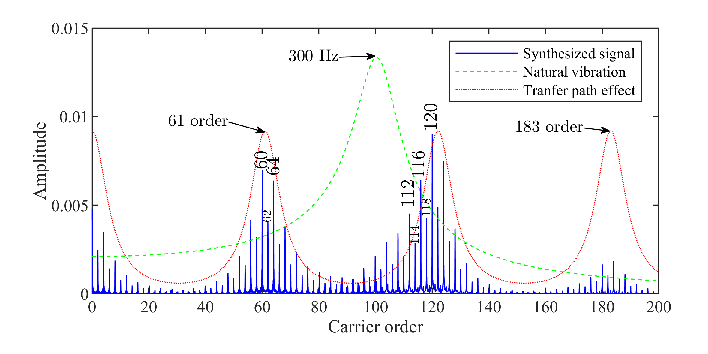
\includegraphics[scale=1]{Shifted_natural_frequency}
    \caption{Spectral surmount cluster shifts towards a higher frequency due to the uneven load distribution of planets}\label{fig:Shifted_natural_frequency}
\end{figure}
\begin{figure}[pos=htbp]
    \centering
    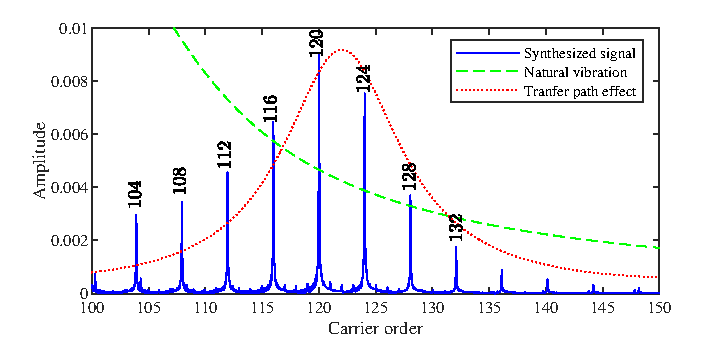
\includegraphics[scale=1]{Figures/4_planet_normal_fourier.pdf}
    \caption{4 planets normal fourier}
    \label{fig:4_planet_normal_fourier}
\end{figure}
\begin{figure}[pos=htbp]
    \centering
    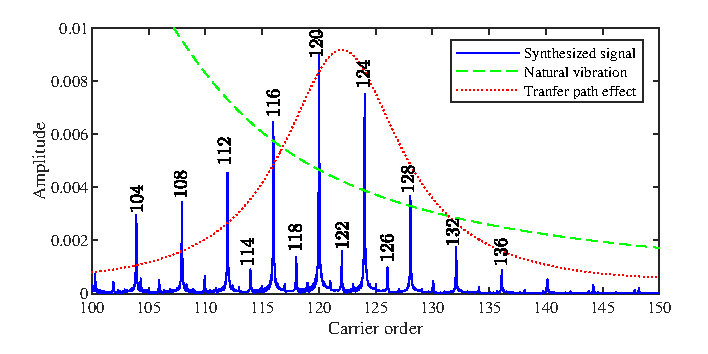
\includegraphics[scale=1]{Figures/4_planet_2-th-0_01_fourier.pdf}
    \caption{4 planets $\epsilon_2=0.01$\degree}
    \label{fig:4_planet_2-th-0_01_fourier}
\end{figure}
\begin{figure}[pos=htbp]
    \centering
    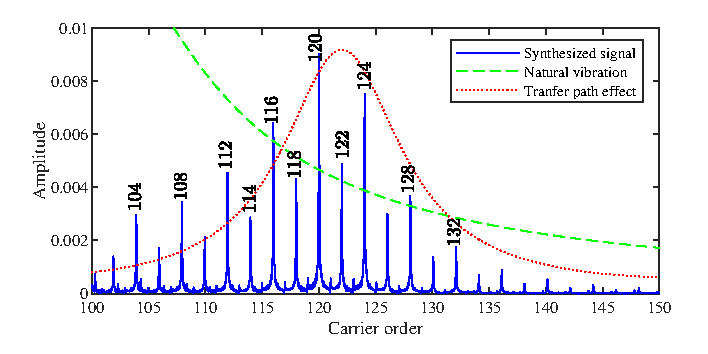
\includegraphics[scale=1]{Figures/4_planet_2-th-0_02_4_th_0_01_fourier.pdf}
    \caption{4 planets $\epsilon_2=0.02$\degree, $\epsilon_4=0.01$\degree}
    \label{fig:4_planet_2-th-0_02_4_th_0_01_fourier}
\end{figure}
\begin{figure}[pos=htbp]
    \centering
    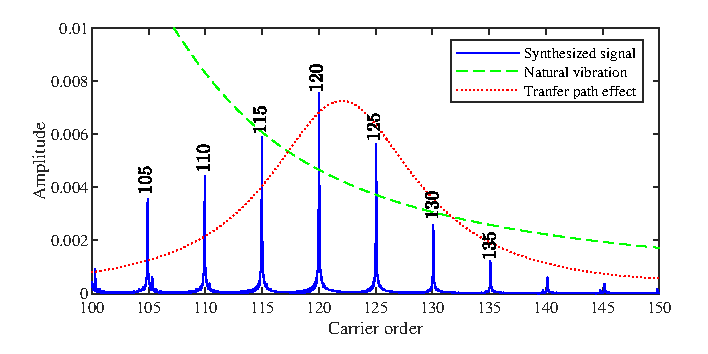
\includegraphics[scale=1]{Figures/5_planet_normal_fourier.pdf}
    \caption{5 planets normal}
    \label{fig:5_planet_normal_fourier}
\end{figure}
\begin{figure}[pos=htbp]
    \centering
    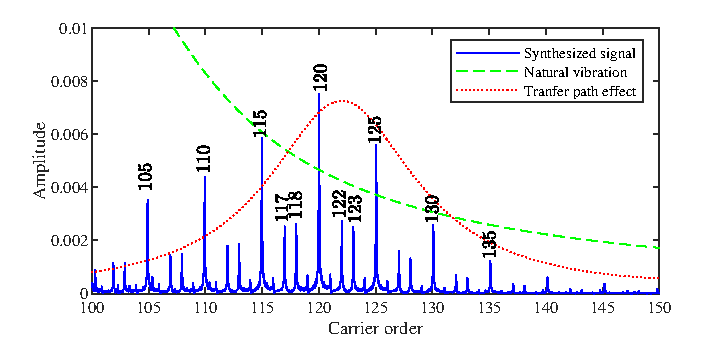
\includegraphics[scale=1]{Figures/5_planet_2_th_0_02_fourier.pdf}
    \caption{5 planets $\epsilon_2=0.02$\degree}
    \label{fig:5_planet_2_th_0_02_fourier}
\end{figure}
\begin{figure}[pos=htbp]
    \centering
    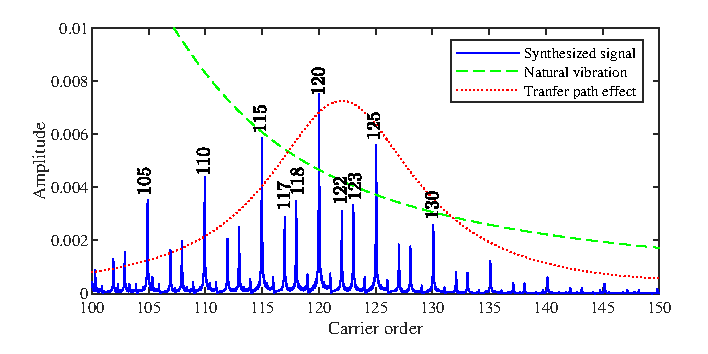
\includegraphics[scale=1]{Figures/5_planet_2_th_0_01_4_th_0_02_fourier.pdf}
    \caption{5 planets $\epsilon_2=0.02$\degree, $\epsilon_4=0.02$\degree}
    \label{fig:5_planet_2_th_0_01_4_th_0_02_fourier}
\end{figure}
\begin{figure}[pos=htbp]
    \centering
    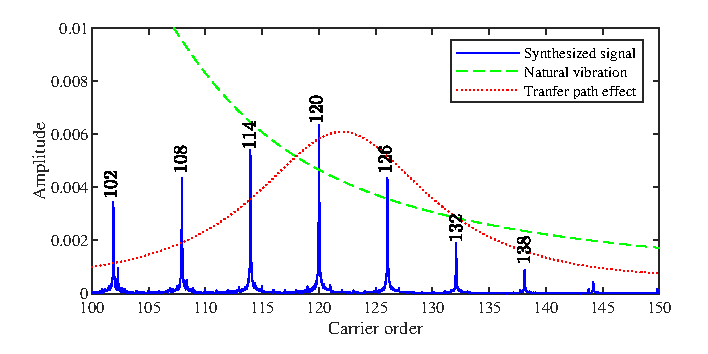
\includegraphics[scale=1]{Figures/6_planet_normal_fourier.pdf}
    \caption{6 planets normal}
    \label{fig:6_planet_normal_fourier}
\end{figure}
\begin{figure}[pos=htbp]
    \centering
    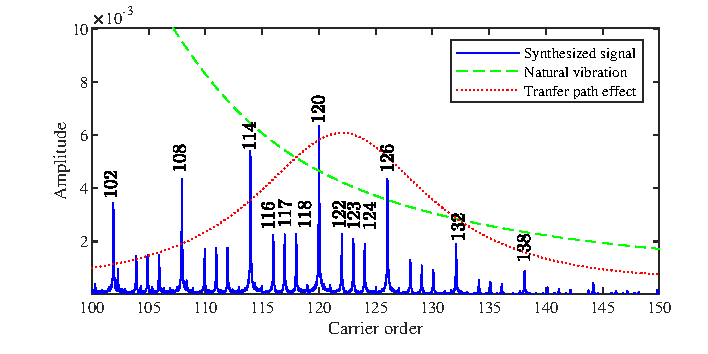
\includegraphics[scale=1]{Figures/6_planet_2_th_0_02_fourier.pdf}
    \caption{6 planets $\epsilon_2=0.02$\degree}
    \label{fig:6_planet_2_th_0_02_fourier}
\end{figure}
\begin{figure}[pos=htbp]
    \centering
    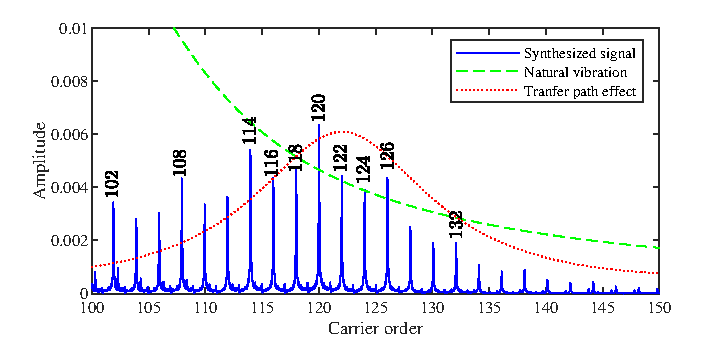
\includegraphics[scale=1]{Figures/6_planet_2_th_0_02_5_th_0.02_fourier.pdf}
    \caption{6 planet $\epsilon_2=0.02$\degree, $\epsilon_5=0.02$\degree}
    \label{fig:6_planet_2_th_0_02_5_th_0.02_fourier}
\end{figure}
\section{Factors considered in the signal model}
\begin{enumerate}
    \item Mechanism of time-varying gear meshing stiffness and risen impulses. (Including sun-planet and ring-planet)
    \item Transfer path effect led by the carrier rotation. \textbf{We now use the exponential attenuation function}
    \item Unequal load sharing risen by the planet angular position error.
    \item Differences in the impulsive intensity of planets with sun and ring gears arisen from the position errors of planet. (Amplitude modulation of angular position error)
    \item Phase shifts of transfer path effect of planet position error. (Frequency modulation of angular position error)
    \item Effects of asynchronous meshing between sun-planet and ring-planet \cite{Parker2004}.
    \item Effects of asynchronous meshing among sun-planets or ring-planets \cite{Inalpolat2009}.
    \item Natural vibration influence on spectral structure.
\end{enumerate}
%%%%%%%%%%%%%%%%%%%%%%%%%%%%%% Appendix %%%%%%%%%%%%%%%%%%%%%%%%%%%%%
\section*{Appendix\label{Appendix}}
\begin{figure}[pos=htbp]
    \centering
    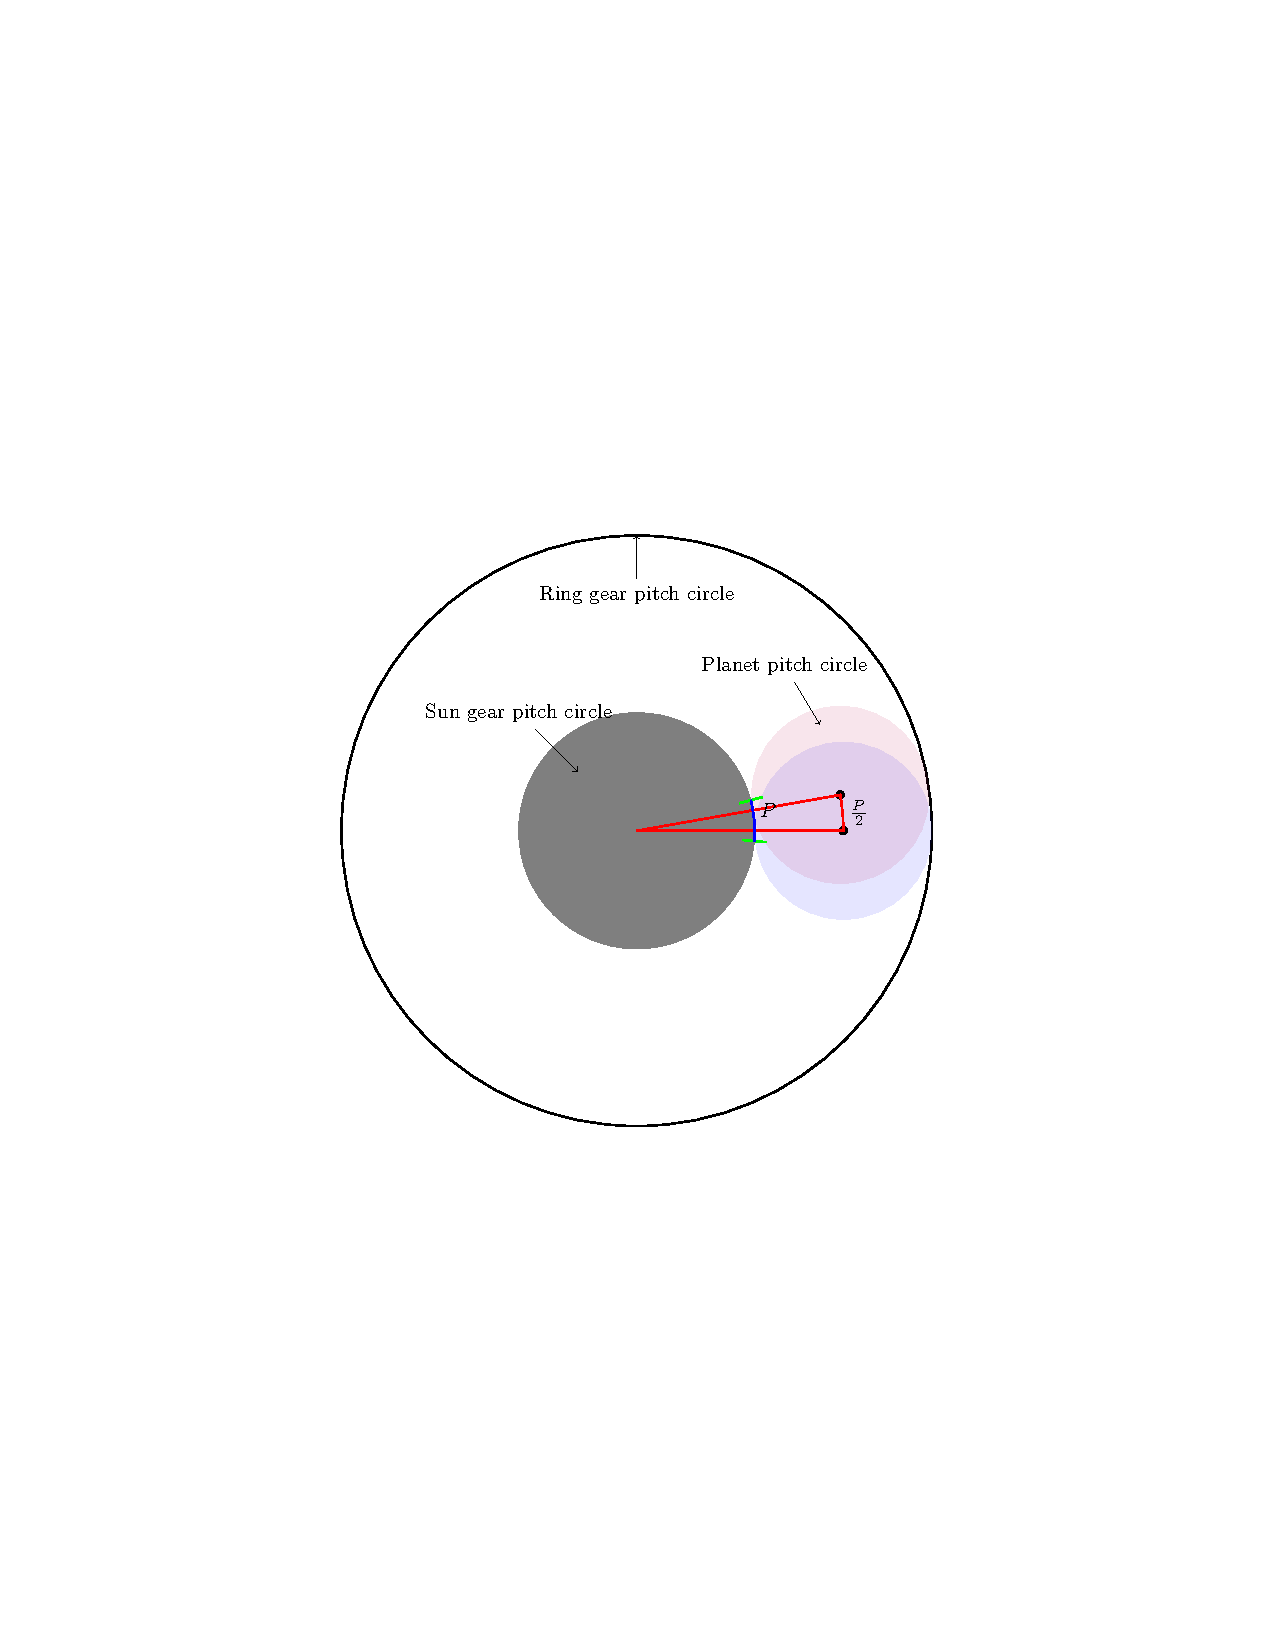
\includegraphics[scale=0.5]{Minimum_angle.pdf}
    \caption{The minimum angle between two adjacent planet possible positions}
    \label{fig_mini_angle}
\end{figure}
\par As shown in Fig. \ref{fig_mini_angle}. The pitch circle of planet gear rolls along the pitch circle of sun gear. When sun gear and ring gear are both fixed, the planet can only assembled at finite discrete angular positions. The minimum angular between two adjacent positions can be calculated as follows. Imagine the sun gear `rotates' an entire tooth, and a planet rotates a distance along with the pinhole circle on the carrier. The transmission ratio between carrier and sun gear is
\begin{equation}
    \operatorname{Transmission\,ratio}=\frac{Z_{\rm s}}{Z_{\rm s}+Z_{\rm r}}
\end{equation}
the angle the sun gear rotates is:$\frac{P}{R_{\rm s}}$, where $P$ is the tooth spacing (base pitch). So the distance the pinhole center rotates is
\begin{equation}
    (R_{\rm s}+R_{\rm p}) \cdot \frac{P}{R_{\rm s}} \cdot \frac{Z_{\rm s}}{Z_{\rm s}+Z_{\rm r}}
    =\frac{R_{\rm s}+R_{\rm p}}{R_{\rm s}+R_{\rm r}} \cdot P
    =\frac{R_{\rm s}+R_{\rm p}}{R_{\rm s}+R_{\rm s}+2R_{\rm p}} \cdot P
    =\frac{P}{2}
\end{equation}
Thus, the angle the planet-carrier rotates is
\begin{equation}
    \lambda=\frac{P}{2} \cdot \frac{1}{R_{\rm p}+R_{\rm s}}
    =\frac{P}{R_{\rm r}+R_{\rm s}}
    \label{equ_carrier_angle}
\end{equation}
According to the definition of module of gear$m=\frac{D}{Z}=\frac{P}{\pi}$, the Eq. (\ref{equ_carrier_angle}) can be rewritten as:
\begin{equation}
    \lambda=\frac{P \cdot 2}{D_{\rm r}+D_{\rm s}}
    =\frac{2 \pi m}{m \cdot ({Z_{\rm r}}+Z_{\rm s})}
    =\frac{2 \pi}{Z_{\rm r}+Z_{\rm s}},
\end{equation}
The planets can only locate finite angular positions with minimum space $\lamda$. When planets locate uniformly at angular positions $\frac{2\pi(i-1)}{M}$, the $Z_{\rm r}+Z_{\rm s}$ must be an integer multiple of planet number $M$.
%% `Elsevier LaTeX' style
\bibliographystyle{elsarticle-num}
\bibliography{My_EndNote_Lib.bib}

\end{document}